\documentclass[]{AVSSimReportMemo}

\usepackage{cite}
\usepackage{AVS}

\usepackage{listings}
\usepackage{color}
\usepackage{ textcomp }

\usepackage{siunitx}
\sisetup{output-exponent-marker=\textsc{e}}

\definecolor{dkgreen}{rgb}{0,0.6,0}
\definecolor{gray}{rgb}{0.5,0.5,0.5}
\definecolor{mauve}{rgb}{0.58,0,0.82}

\lstset{frame=tb,
  language=Python,
  aboveskip=3mm,
  belowskip=3mm,
  showstringspaces=false,
  columns=flexible,
  basicstyle={\small\ttfamily},
  numbers=none,
  numberstyle=\tiny\color{gray},
  keywordstyle=\color{blue},
  commentstyle=\color{dkgreen},
  stringstyle=\color{mauve},
  breaklines=true,
  breakatwhitespace=true,
  tabsize=3
}


\newcommand{\ModuleName}{integrator}
\newcommand{\subject}{Integrator architecture in C++ and Python}
\newcommand{\status}{Tested}
\newcommand{\preparer}{M. Diaz Ramos}
\newcommand{\summary}{Integrator architecture model and implementation are described.}


\begin{document}


\makeCover


%
%	enter the revision documentation here
%	to add more lines, copy the table entry and the \hline, and paste after the current entry.
%
\pagestyle{empty}
{\renewcommand{\arraystretch}{2}
\noindent
\begin{longtable}{|p{0.5in}|p{4.5in}|p{1.14in}|}
\hline
{\bfseries Rev}: & {\bfseries Change Description} & {\bfseries By} \\
\hline
1.0 & First version & M. Diaz Ramos \\
\hline

\end{longtable}
}

\newpage
\setcounter{page}{1}
\pagestyle{fancy}

\tableofcontents
~\\ \hrule ~\\

\section{Introduction}

An integrator architecture model is described. How to use and create new integrators is shown.

\section{Document ID}
{\tt AVS-SIM-\ModuleName}.  

\section{The model}

The model is shown in Figure \ref{fig:class}. The architecture is structured around two very simple abstract classes: \textit{integrator} and \textit{dynModel}. The former defines the simple interface \textit{integrate()}, while the latter defines \textit{equationsOfMotion()}. An integrator just uses the \textit{integrate()} method to advance one time step using the dynamics defined by \textit{equationsOfMotion()} (also known as the $F$-function in the dynamics equation $\dot X = F(X, t)$).

\begin{figure}
\centering
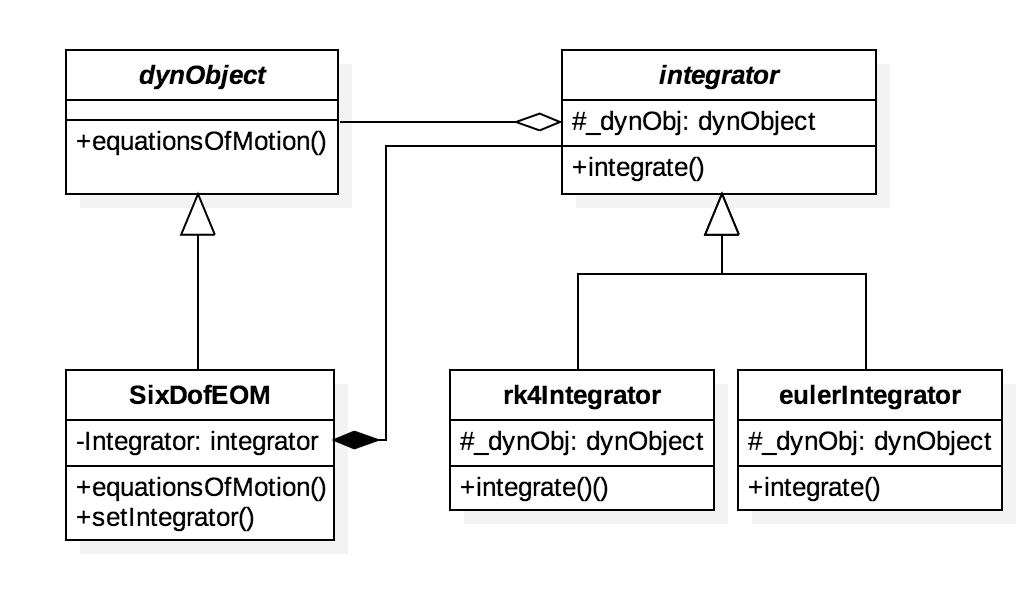
\includegraphics[width=0.7\textwidth]{Figures/class_diagram.png}
\caption{UML class diagram.}\label{fig:class}
\end{figure}

In order to create a new integrator, just inherit the abstract class \textit{integrator} and implement the \textit{integrate()} method.

The integrator can be used by calling \textit{SixDofEOM::setIntegrator()}.

The following snippet shows how to use an Euler integrator in Python.
\begin{lstlisting}
sixDofObj = six_dof_eom.SixDofEOM()
eulerInt = six_dof_eom.eulerIntegrator(sixDofObj)
sixDofObj.setIntegrator(eulerInt)
\end{lstlisting}



\end{document}
